\chapter{Structure of CoCos}

\section{Description of CoCos}

\section{Payoff and Risk Profile}

\begin{figure}[ht]
	\centering
	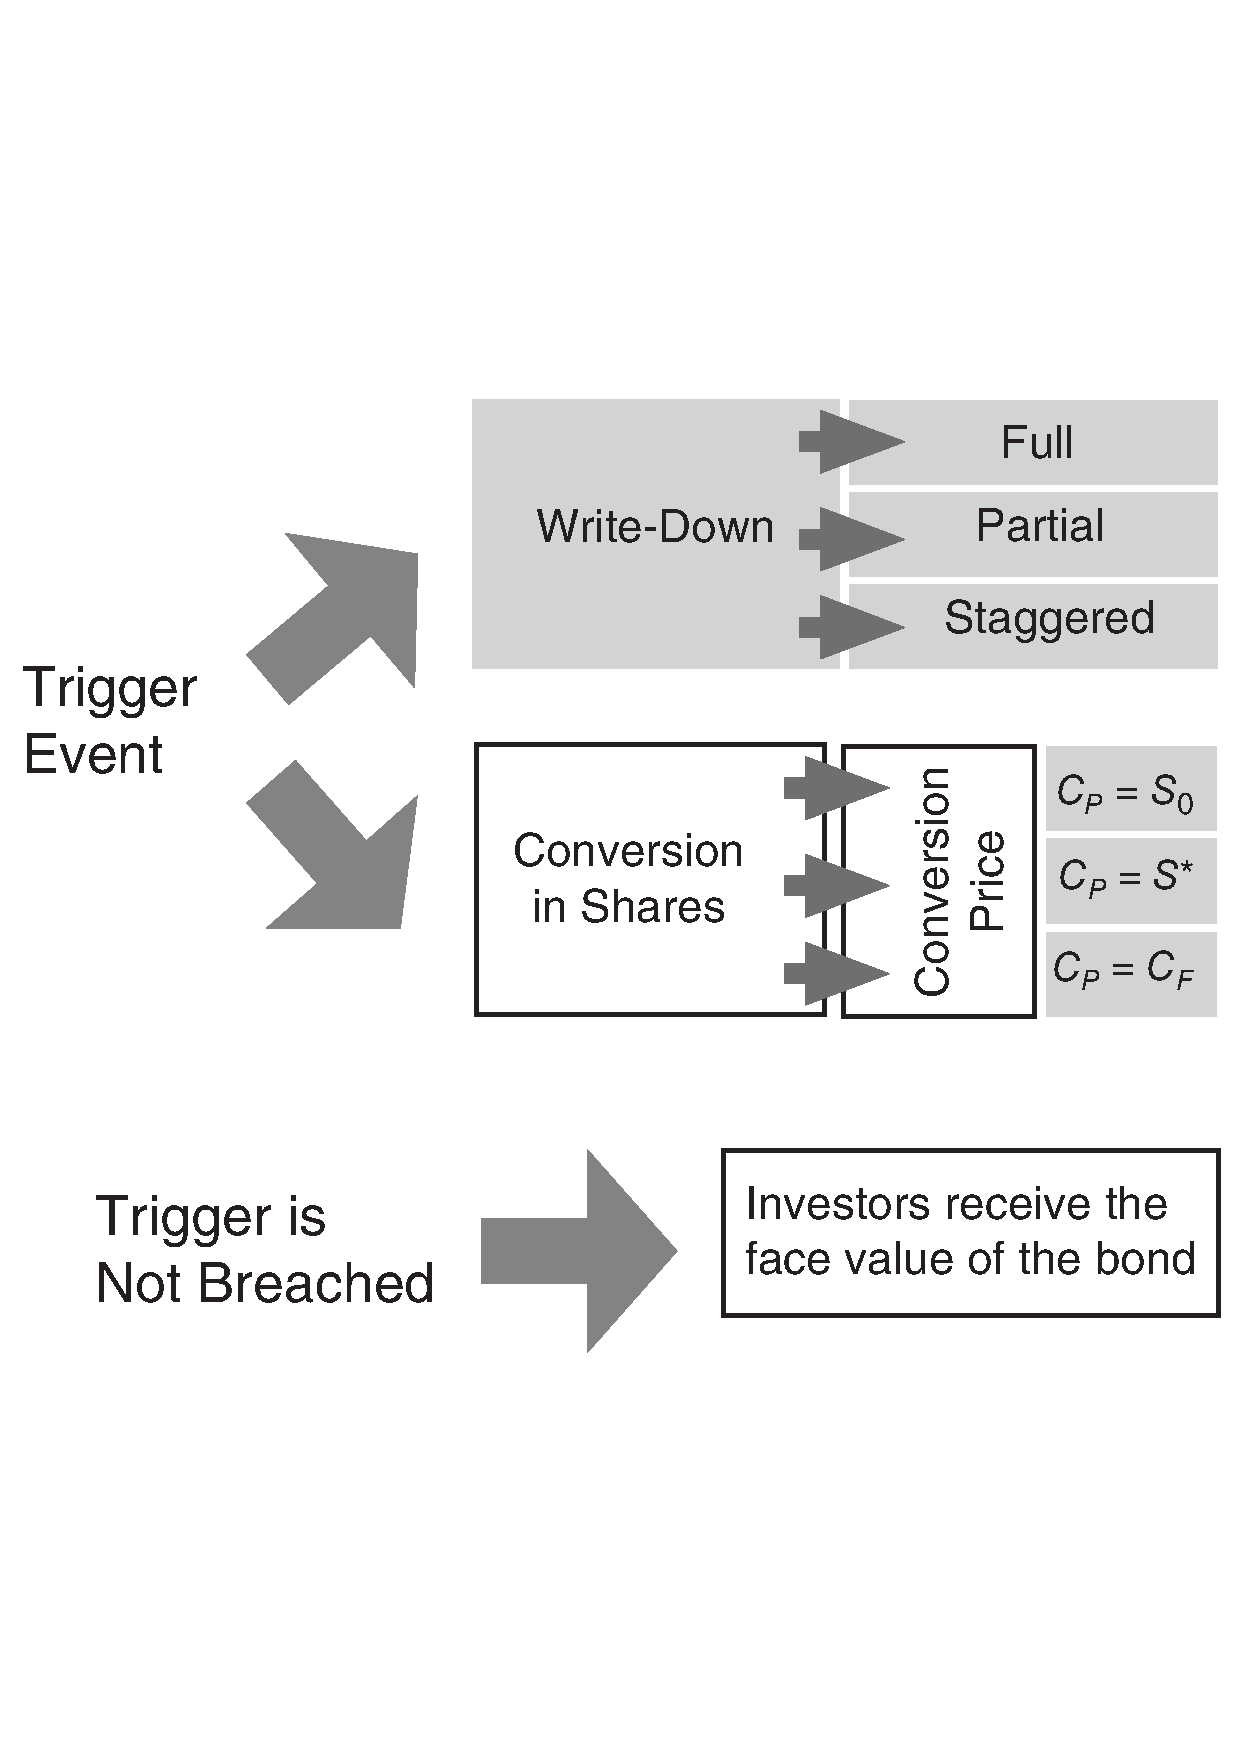
\includegraphics[trim=0.6cm 7.05cm 0.9cm 7cm, scale = 0.4]{media/anatomy} \par
	\caption{Anatomy of Cocos \citep{de2011handbook}}
\end{figure}
asdasd

\section{Conversion Trigger}

\subsection{Market Trigger}

\subsection{Accounting Trigger}

\subsection{Regulatory Trigger}

\subsection{Multivariate Trigger}

\section{Conversion Details}

\subsection{Conversion Fraction}

\begin{itemize}
    \item conversion fraction $\alpha$
    \item face value $N$
    \item conversion amount $N \times \alpha$
    \item amount remaining in case of partial equity conversion $N \times (1-\alpha)$
\end{itemize}

\subsection{Conversion Price and Ratio}
%test
\begin{itemize}
    \item conversion rate $C_r$
    \item conversion price $C_p$
    \item recovery rate $R_{CoCo}$
    \item stock price at trigger event $S_T^{*}$
    \item loss attributable to CoCo holders $L_{CoCo}$
\end{itemize}

\begin{align}
    C_p &= \frac{\alpha N}{C_r}\\
    C_r &= \frac{\alpha N}{C_p}\\
    R_{CoCo} &= \frac{S_T^{*} }{C_p}\\
    L_{CoCo} &= N - ( 1 - R_{CoCo}) = N \left( 1 - \frac{S_T^{*}}{C_p} \right)\\
    P_T &= \begin{cases} (1 - \alpha) N + C_r S_T^{*} & \text{ if converted} \\ N & \text{if not converted} \end{cases}
\end{align}

